% =============================================================================
% Chapter 6 — The Patch Train: Fail-Closed Runtime Surgery
% Sources: book-notes/patches-digest.md, book-notes/scripts-digest.md,
%          repo docker-compose.dspark.yml (entrypoint), CHANGELOG.md,
%          docs/PATCHES.md
% =============================================================================

\chapter{The Patch Train: Fail-Closed Runtime Surgery}
\label{ch:patches}

Until the 2026-08-22 fail-closed conversion (issue \ghissue{107}), this
deployment's boot sequence contained a quiet trap: its default-on Python
patchers were separated by \emph{bare semicolons} in the container
entrypoint, so a missing patch file, an anchor drift, or a failed self-check
was masked by the next successful command. The server started anyway,
serving stale runtime code with every appearance of a clean boot. The
principle the fix encoded is the thesis of this chapter: \emph{an enabled
boot must never silently serve stock behavior.}

The trap existed because of a question every inference deployment that pins a
third-party runtime image eventually faces: the image has bugs, upstream has
fixes (or you have written your own), and the model must keep serving. This
repository's answer is a corpus of more than forty patch files that rewrite
the installed vLLM tree \emph{inside the container, at every boot, before}
\code{exec vllm serve} --- a ``patch train'' that either delivers a
byte-verified runtime or refuses to start at all. This chapter is about the
method, not the individual bugs (those are the subject of \Cref{ch:bugs}):
how the patchers are structured, how they are gated, how independent fixes
compose on the same files, and how a CPU-only CI gate keeps the whole
apparatus honest.

For an inference engineer, this is the most transferable material in the book
--- any team running a pinned engine image on hardware upstream does not test
will end up building something like it. This repository shows what the mature
form looks like: fail-closed gating, byte-exact provenance, and rollback by
recreation rather than by hope.

\section{The strategic choice: patch a pinned image at boot}
\label{sec:patches-strategy}

The deployment target throughout is one image, pinned by registry manifest
digest:

\begin{lstlisting}
ghcr.io/anemll/dspark-vllm-gx10:0.1.1
  @sha256:a83948492cf13df455170fb42885f5ef4db54fefe0feff0f841ecbff464ac9d8
  -> config/image ID sha256:3430d6614a8e2925f34d059af6caf05aff42387326db4d05639a60f10f2654d8
carrying vLLM 0.25.2.dev0+g752a3a504.d20260714
installed at /usr/local/lib/python3.12/dist-packages/vllm
\end{lstlisting}

The obvious alternative --- fork the image, apply the fixes at build time, and
ship a rebuilt image --- was rejected. Patch-at-boot buys three things the
fork cannot easily provide:

\begin{itemize}
\item \textbf{Byte-exact provenance.} The runtime tree at any moment is a pure
  function of two published artifacts: the pinned digest and the patch corpus.
  Several patchers make this literal, pinning the SHA-256 of the file they
  expect to find and of the file they leave behind, so ``what code is this
  rank actually running?'' has a checkable answer.
\item \textbf{Tiny, reviewable diffs.} Each fix is one file with its own
  docstring, evidence, marker, and \code{--status} mode --- not a commit
  buried in an image rebuild. The whole train is legible in the compose
  entrypoint.
\item \textbf{Rollback by recreation.} Because patches live only in the
  container's writable layer, discarding the container (\code{docker rm} and
  a fresh \code{create}) restores the pristine pinned image exactly. Turning
  a fix off is a flag flip plus a recreate --- no image rebuild, no registry
  round-trip.
\end{itemize}

The costs are real and the repository documents them bluntly. Patched bytes live in
the writable layer, so the layer becomes hidden state: a plain
\code{docker restart} \emph{keeps} whatever the previous boot wrote.
\repofile{docs/PATCHES.md} states the doctrine for the \ghissue{136}
patcher in one sentence: ``\code{docker restart} or restarting the process
reuses the patched writable layer and is \textbf{not} rollback.'' Every
flag change therefore requires a paired stop/remove/start on both nodes.
The patchers themselves must be engineered to meet a tree that some earlier
boot already modified --- which is why idempotence, drift detection, and
multi-pre-image pinning (\Cref{sec:patches-compose}) are first-class problems
here rather than afterthoughts (\Cref{fig:patch-writable-layer}).

\begin{hbwarstory}
The TP=3 patcher learned the writable-layer lesson ``the hard way.'' Its
idempotence markers were originally derived from each edit's description
alone, so when a patch \emph{body} changed, a container whose writable layer
held the \emph{old} body still looked ``already patched.'' The stale
code survived every compose restart, with the only symptom a shape assert on
rank 2. The fix: markers now embed a SHA-256 prefix of the replacement body.
A stale body yields a \code{STALE} verdict, which is a hard exit-1 failure
with explicit remediation --- \code{docker rm -f} on every node, because the
anchor has been consumed and the file cannot be re-anchored in place.
\end{hbwarstory}

\begin{figure}[htbp]
\centering
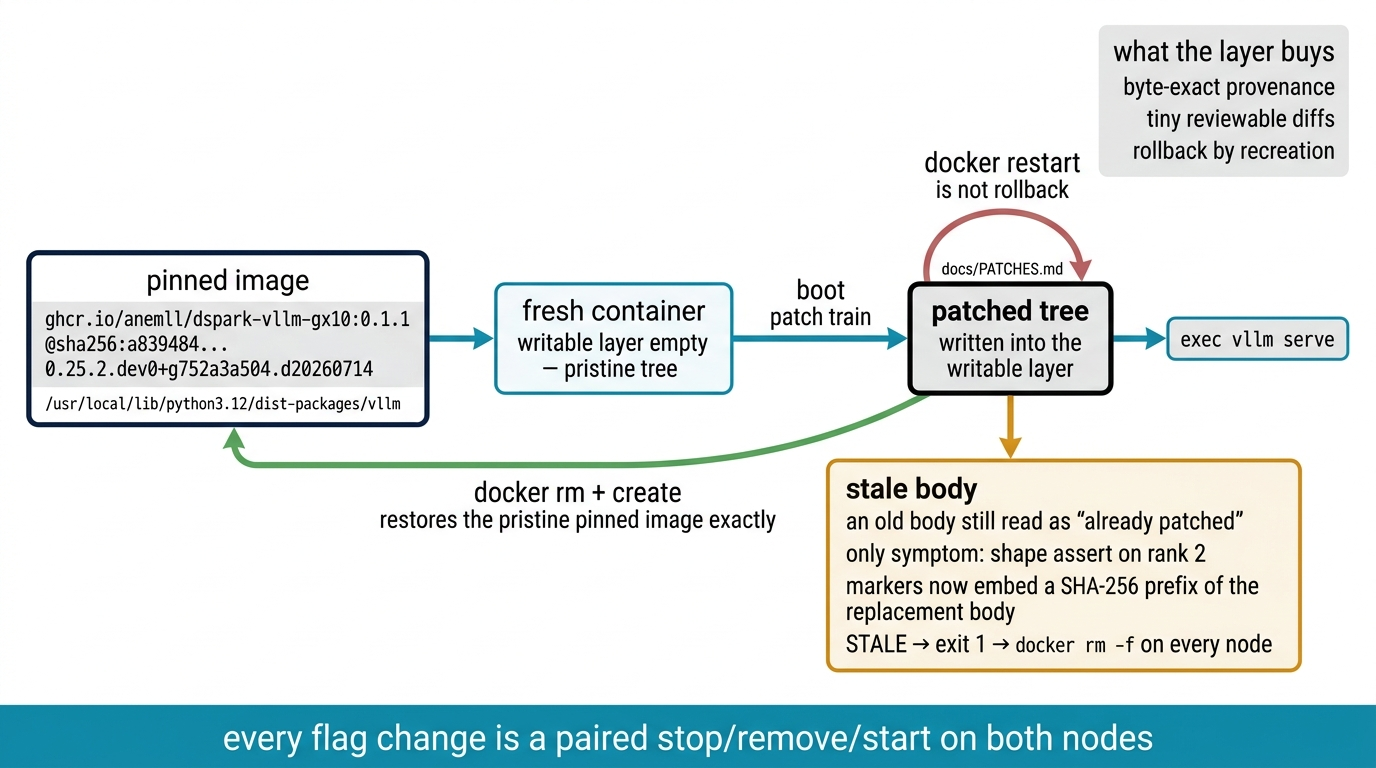
\includegraphics[width=\textwidth]{figures/ch06-restart-not-rollback.png}
\caption{Patched bytes live only in the container's writable layer. That is
what makes rollback a recreate rather than an image rebuild --- but it also
makes the layer hidden state: \code{docker restart} reuses whatever the
previous boot wrote and is not rollback, so every flag change is a paired
stop/remove/start on both nodes. The TP=3 patcher learned the corollary the
hard way: idempotence markers derived from an edit's description alone let a
stale body still read as ``already patched'', surviving every compose restart
with a shape assert on rank 2 as the only symptom. Markers now embed a
SHA-256 prefix of the replacement body, and a stale body is a hard
\code{STALE} exit 1 demanding \code{docker rm -f} on every node.}
\label{fig:patch-writable-layer}
\end{figure}

\section{Four patcher families}
\label{sec:patches-families}

The corpus that grew up under these constraints --- idempotence against a
dirty writable layer, drift detection, stale-body refusal --- is not
uniform: it shows an escalating ladder of verification rigor matched to
blast radius. \Cref{tab:patch-families} summarizes the four
recognizable families; the subsections that follow give one worked example of
each.

\begin{table}[htbp]
\centering
\small
\caption{The four patcher families, ordered by verification rigor.}
\label{tab:patch-families}
\begin{tabular}{>{\raggedright\arraybackslash}p{3.4cm}>{\raggedright\arraybackslash}p{4.3cm}>{\raggedright\arraybackslash}p{3.2cm}>{\raggedright\arraybackslash}p{3.2cm}}
\toprule
Family & Integrity mechanism & Failure handling & Examples \\
\midrule
Anchor+marker Python startup patchers & exact-anchor match, occurrence
  counts, \code{compile()} before write, marker comment & exit 1 on
  anchor drift; idempotent re-runs & \ghissue{27}, \ghissue{43},
  \ghissue{26} v2, \ghissue{133}, adaptive chunk \\
Transactional multi-hunk shell backports & staged in-memory view; all hunks
  validate before any write; atomic per-file rename & post-commit byte
  verify; reverse-order rollback of published files & upstream PRs
  \ghissue{48407}, \ghissue{48957}, \ghissue{49486}, \ghissue{50298},
  \ghissue{50312}, \ghissue{44993} \\
SHA-256 pre/post-image patchers & whole-file or AST-extracted-method hash
  pins; version pins; TOCTOU stat guards & staged rollback image; verified
  restore; loud exit 2 if restore fails & \ghissue{117}, \ghissue{136}/210,
  \ghissue{138}, codex, \ghissue{141}, block-k, responses store \\
Overlay packages and reference patches & normal Python import (via an
  appended hook) or plain unified diff & fail-closed installer; diffs
  are documentation or build-time & \repofile{vision_exp/}, \repofile{tp3/},
  three \code{.patch}/\code{.diff} files \\
\bottomrule
\end{tabular}
\end{table}

\subsection{Anchor+marker startup patchers}

The workhorse family: idempotent Python scripts that match \emph{exact stock
source text}, replace it once, syntax-check the result, and write back. The
shape, common to a dozen scripts, is:

\needspace{12\baselineskip}
\begin{lstlisting}[language=Python]
# representative shape (pseudocode distilled from the family)
src = target.read_text()
if MARKER in src:            # idempotent: an earlier boot already patched
    verify_and_exit(0)
assert src.count(OLD) == 1   # anchor drift or ambiguity -> SystemExit(1)
patched = src.replace(OLD, NEW_WITH_MARKER, 1)
compile(patched, str(target), "exec")   # syntax gate BEFORE any write
target.write_text(patched)
# every script also answers --status: APPLIED / NOT APPLIED / stale states
\end{lstlisting}

A representative member is
\repofile{patches/hotfix-dsv4-adaptive-prefill-chunk.py} (67 lines): it
anchors the two chunk-cap sites in the v1 scheduler, asserts both anchors are
present, widens the cap logic so a cold single-request prefill is not chunked,
compiles before writing, and tags its work with the marker comment
\code{[dspark-adaptive-chunk]}.

The family also supports \emph{revisioned}
patches: the \ghissue{27} scheduler patcher carries r3 markers and
refuses with exit 1 if it finds an older r2 application, because the r2
anchors were consumed and only a pristine file can be re-patched. It reports
\code{APPLIED (r2, stale)} rather than guessing. The most interesting member,
the \ghissue{26} hotfix, is a patcher that \emph{reverts its own v1}:
its \code{apply_text()} recognizes three file states (stock, v1-injected,
already-v2) and replaces an in-image v1 injection with the corrected v2
block, since v1 had caused warm-prefix garbage (\Cref{ch:bugs}).

\subsection{Transactional multi-hunk shell backports}

The upstream-PR backports (\ghissue{48407}, \ghissue{48957}, \ghissue{49486},
\ghissue{50298}, \ghissue{50312}, \ghissue{44993}) each change several hunks
across one to four files, and a partially applied backport would be worse than
none. The family's answer is to take the database vocabulary literally: a
backport is a transaction over files, and atomic per-file rename is enough
primitive to build one. Each is a bash wrapper around an embedded Python ``whole-script
transaction'': every hunk validates against an in-memory staged view of its
target, and nothing touches disk until \emph{all} hunks validate and compile.
Publication is per-file atomic (\code{mkstemp} in the same directory,
\code{fsync}, \code{os.replace}, directory \code{fsync}), and the committed
bytes are re-read and verified. Any failure rolls back every
already-published file in reverse order --- with a nonzero, loud exit if the
rollback itself fails. Per-hunk state is a
\code{count(old)}/\code{count(new)} machine: $(1,0)$ applies, $(0,1)$ is
already patched, anything else is refused as ambiguous. A
\code{_track_published} guard even covers the race where an interrupt lands
after the rename syscall but before bookkeeping. \Cref{fig:patch-transaction}
draws the state machine.

The worked example is
\repofile{patches/hotfix-dsv4-flashmla-workspace-50298.sh} (542 lines,
six hunks across two files): it backports upstream vLLM PR \ghissue{50298},
which removed a per-chunk \code{torch.full(-1)} allocation on the sparse
prefill path by reserving the two int32 index buffers in the capture-time
workspace and threading an \code{out=} parameter through
\code{combine_topk_swa_indices()}. Six edits, two files, one transaction:
either both files end up in the post-image state, or neither does.

\begin{figure}[htbp]
\centering
\begin{tikzpicture}[node distance=4.5mm and 8mm]
  % idempotent shortcut (left column)
  \node[hbfaint, text width=2.9cm] (idem)
    {already patched:\\ \scriptsize re-verify only,\\ \scriptsize no write};
  % main pipeline (center column)
  \node[hbnode, text width=4.4cm, right=16mm of idem] (val)
    {\textbf{1.\ validate pre-image}\\ \scriptsize SHA-256 / anchor-count state
     machine over a staged in-memory view; ambiguity refused};
  \node[hbnode, text width=4.4cm, below=of val] (build)
    {\textbf{2.\ build + compile}\\ \scriptsize all candidate files constructed
     and syntax-checked in memory; nothing written yet};
  \node[hbnode, text width=4.4cm, below=of build] (stage)
    {\textbf{3.\ stage}\\ \scriptsize same-directory temp file,
     mode preserved, fsync};
  \node[hbbox, text width=4.4cm, below=of stage] (rename)
    {\textbf{4.\ publish}\\ \scriptsize atomic os.replace + directory fsync,
     file by file in order};
  \node[hbnode, text width=4.4cm, below=of rename] (verify)
    {\textbf{5.\ re-verify}\\ \scriptsize re-read published bytes:
     hash, mode, compile};
  \node[hbgpu, text width=4.4cm, below=of verify] (ok)
    {\textbf{committed} --- exit 0};
  % rollback column (right)
  \node[hbwarn, text width=3.6cm, right=of rename] (rb)
    {\textbf{rollback}\\ \scriptsize restore every published file in
     \emph{reverse} order from staged rollback images};
  \node[hbwarn, text width=3.6cm, below=of rb] (rbver)
    {restore verified\\ \scriptsize exit 1 --- boot blocked};
  \node[hbwarn, text width=3.6cm, below=of rbver] (fatal)
    {rollback failed\\ \scriptsize loud FATAL --- exit 2};
  % flows
  \draw[hbflow] (val) -- (build);
  \draw[hbflow] (build) -- (stage);
  \draw[hbflow] (stage) -- (rename);
  \draw[hbflow] (rename) -- (verify);
  \draw[hbok]   (verify) -- (ok);
  \draw[hbarrow] (val) -- node[hblabel, above, font=\tiny]{post-image} (idem);
  \draw[hbok]   (idem.west) -- ++(-5mm,0) |- (ok.west);
  \draw[hbfail] (rename.east) -- node[hblabel, pos=0.4, above=0.5mm,
    font=\tiny, fill=white, inner sep=1pt]{publish fails} (rb.west);
  \draw[hbfail] (verify.east) -- (rb.south west);
  \draw[hbfail] (rb) -- (rbver);
  \draw[hbfail] (rbver) -- node[hblabel, right]{restore mismatch} (fatal);
  \node[hblabel, text width=2.6cm, align=center, below=4mm of idem] (drift)
    {drift / ambiguity:\\ exit 1, no write};
  \draw[hbfail] (val.south west) to[bend right=15] (drift.north);
\end{tikzpicture}
\caption{The transactional patcher state machine shared by the multi-hunk
backports and the SHA-pinned family. Failures in steps 1--2 exit before any
write; failures at publish or verification trigger a verified reverse-order
restore of everything already published. An already-patched target takes the
idempotent path: re-verify, never rewrite.}
\label{fig:patch-transaction}
\end{figure}

\subsection{SHA-256 pre/post-image patchers}

The strictest family locks the \emph{complete file} (or a complete
AST-extracted method) by SHA-256 pre-image and post-image, refuses any drift,
stages a rollback image before touching the target, and verifies bytes, mode,
and source state after publication. The bounded Responses-store patcher is the
canonical whole-file example. Its contract, published verbatim in
\repofile{docs/PATCHES.md}:

\needspace{6\baselineskip}
\begin{lstlisting}
/usr/local/lib/python3.12/dist-packages/vllm/entrypoints/openai/responses/serving.py
stock SHA-256   fe3a48ab09c516835ce6dd1471c06cc784ae7504eaa7af7f10574704106830d8
patched SHA-256 1b0033131a34e03a2e129743258f5da81b3e60e979072920153f6d09bf4e5d8f
\end{lstlisting}

Fourteen named anchor$\rightarrow$replacement pairs are applied in order, and
the result must hash to the pinned post-image before an atomic publish. The
transform turns vLLM's self-described leak (``may cause a memory leak since we
never remove responses from the store'') into an LRU-bounded store capped by
\envvar{DSPARK_RESPONSES_STORE_MAX_ENTRIES} (default 256). The extreme of
whole-file pinning is the \ghissue{117} patcher: four pinned
whole-file identities, a TOCTOU guard that \code{lstat}s the target before
and after reading it, a rename-race probe, and a rollback that re-verifies
bytes, metadata, state, and compilation.

The \ghissue{138} and codex patchers refine the granularity: rather
than pinning a whole file that other patches may legitimately touch, they use
\code{ast.parse} to extract the one \code{input_item_parsing} method from
\repofile{entrypoints/openai/responses/protocol.py}, require the extracted
text to occur exactly once, and pin \emph{that method's} SHA-256 (old
\code{2412484a...}, expected new \code{536f3a30...}) plus two ordered
outer guards --- a method-granular source lock that survives changes elsewhere
in the file.

Several members also pin the environment itself: the block-k patcher
requires the installed vLLM version string to equal
\code{0.25.2.dev0+g752a3a504.d20260714} via \code{importlib.metadata}, and
the \ghissue{136} chain pins the \code{xgrammar} version (0.2.3) as
well.

The \ghissue{141} workaround pushes pinning across a package
boundary. Its correctness argument rests on the pinned FlashInfer revision's
dispatch contract --- calls of at most 64 rows take the standalone DSv4
decode kernel. The patcher therefore pins exact guard fragments from FlashInfer
itself: the 64-row cutoff in the workspace helper, the
\code{_DECODE_MAX_TOKENS = 64} definition, the dispatch predicate, the
adapter call signature, and the custom-op \code{mutates_args} contract that
excludes both KV caches. Each fragment must occur exactly once \emph{and in
pinned relative order} --- the check verifies offset monotonicity, so even
guard \emph{reordering} counts as drift. The patcher thereby verifies not
just the code it rewrites but the code its justification depends on.

What escalates across this family is scope rather than strictness: from the
bytes of a whole file, to the bytes of one extracted method, to the installed
version string, to fragments of a different package whose behavior the fix's
correctness argument rests on.

\subsection{Overlay packages and reference patch files}

Not everything is an in-place rewrite. \repofile{patches/vision_exp/} is a
normal Python package (ViT + Aligner model, image processor, vLLM multimodal
processor, and a monkey-patch layer) that the installer
\repofile{patches/hotfix-dsv4-vision-exp.py} wires in by \emph{appending} a
fail-closed import hook to the stock \repofile{nvidia/model.py}. The stock
classes are passed into \code{apply_vision_exp()} and grafted, never edited
wholesale. \repofile{patches/tp3/apply_tp3_patch.py} is a self-contained
multi-edit patcher (741 lines, eleven edits plus a generated pad module) for
the optional three-node topology. And three plain \code{.patch}/\code{.diff}
files round out the corpus: a 22-line unified diff that is the documentation
twin of the executable \ghissue{22} hotfix, a git diff against the
recipe's own overlay (the draft-KV concurrency fix), and the large
upstream-facing diff carrying the \code{nvfp4_ds_mla} KV dtype and the B12X
MoE backend. Reference diffs matter in this method: they are the reviewable,
upstreamable statement of intent that the executable patchers implement.

\section{The gating doctrine}
\label{sec:patches-gating}

A rigorous patcher is still only as trustworthy as its invocation --- the
bare-semicolons trap that opened this chapter was an invocation failure, not
a patcher failure. \Cref{fig:patch-train} shows the boot sequence the
compose entrypoint actually runs. The governing rules are few and absolute.

\textbf{Exact-\code{"1"} opt-in.} Every gated patcher runs only when its
environment flag compares equal to the literal string \code{1}. Unset,
\code{0}, \code{true}, \code{yes}, or a stray space all mean \emph{stock
behavior} --- there is no truthiness parsing to get wrong:

\begin{lstlisting}[language=bash]
if [ "${DSPARK_ENABLE_ISSUE136_XGRAMMAR_HOTFIX:-0}" = "1" ]; then
  python3 /opt/hotfix-vllm-issue136-xgrammar-termination.py || exit 1;
fi
\end{lstlisting}

\textbf{Default-off for anything unproven.} The \ghissue{31} GPU
thinking-budget patch and the assistant-final continuation fix both started
life applied by default and were deliberately demoted to opt-in gates ---
the former because leaving it on reproduced a decode cliff for clients that
omit the field, the latter to restore stock rendering as the default. The
\ghissue{141} workaround ships default-\code{0} precisely because the
repository classifies it as ``a workaround, not a root-cause fix'' with live
validation still outstanding. Conversely, always-on fixes get \emph{skip}
switches (\envvar{DSPARK_SKIP_HOTFIX},
\envvar{DSPARK_SKIP_SPIN_WAIT_HOTFIX}), not enable flags. One patch,
the API-key log redaction, gets no bypass at all: keyed boots apply and
verify it outside the skippable loop, so \envvar{DSPARK_SKIP_HOTFIX}\code{=1}
can never expose keys in logs.

\textbf{Fail-closed chaining.} Every invocation is chained with
\code{|| exit 1}, and every missing patch file is a FATAL before the run:

\begin{lstlisting}[language=bash]
# always-on backport train (reformatted from docker-compose.dspark.yml)
if [ "${DSPARK_SKIP_HOTFIX:-0}" != "1" ]; then
  for _hf in hotfix-dsv4-mtp-buffer-50312.sh   hotfix-dsv4-skip-topk-49486.sh \
             hotfix-dsv4-dense-prefill-indexer-48407.sh \
             hotfix-dsv4-skip-empty-c128-48957.sh \
             hotfix-dsv4-flashmla-workspace-50298.sh \
             hotfix-dsv4-grammar-advance.sh; do
    if [ ! -f /opt/dspark-patches/${_hf} ]; then
      echo "FATAL: /opt/dspark-patches/${_hf} missing" >&2; exit 1;
    fi
    bash /opt/dspark-patches/${_hf} || exit 1
  done
fi
\end{lstlisting}

\begin{hbwarstory}
The bare-semicolons trap that opened this chapter (issue \ghissue{107}) is
worth revisiting at the level of its fix. Converting the chain to
\code{|| exit 1} was the visible change; the substance was making failure
\emph{reachable}: \ghissue{21} anchor drift and a missing
suppress-stops target were made to return nonzero in their own right.
CPU failure injection was added covering every step and every ordering, so
a masked failure cannot quietly return. The previous day's entry
(2026-08-21) had already completed the picture for the shell side: the
enabled hotfix train ``aborts before \code{vllm serve} when a script is
missing or exits nonzero,'' and all seven multi-hunk backports became
transactional.
\end{hbwarstory}

\textbf{Two-rank preflight.} For the SHA-pinned opt-ins, the launcher does
not trust boot-time discovery. It syncs the canonical patcher to the worker
over \code{scp} and runs \code{--check} on the \emph{worker, then the head,
before either rank's container starts}. An incompatible tree on either
node therefore aborts the launch while both ranks are still down, rather than
letting one rank boot patched and the other refuse. Each container then re-applies
and re-verifies fail-closed before its own \code{exec}.

\textbf{Truthful \code{--status}.} Nearly every patcher answers
\code{--status}, and the repository holds that output to an unusual standard.

\begin{hblesson}
The API-key redaction patch states the doctrine in its own source:
``a hotfix whose \code{--status} lies is worse than no hotfix.'' Its status
mode is therefore \emph{behavioral}, not textual: beyond checking markers and
asserting the pre-patch logging body is gone, it extracts the injected helper
from the installed bytes, executes it standalone, and proves it actually
redacts. A probe key must be absent from the output, the count-preserving
placeholder (\code{<redacted:2 value(s)>}) must be present, and the live
argument list must not have been mutated. Partial states --- redactor present
but a raw logger reintroduced --- are hard errors. A marker grep tells you a
patch was applied once; a behavioral probe tells you the protection holds
\emph{now}. When a patch guards something that matters (here: secrets in
\code{docker logs}), build the second kind.
\end{hblesson}

\begin{hbnote}
Fail-closed thinking also runs in the opposite direction: shipping machinery
that deliberately cannot fire. The \ghissue{48407} backport
(``skip indexer scoring on short dense prefills'') is installed
\emph{dormant} --- all eleven hunks are applied, but the layer-name binding
that arms the skip is the empty string, which the resolver treats as falsy.
The premise of the upstream fix (a dense-MHA route for short prefills) is
false on this fork, and enabling the skip would silently drop valid KV
selection. Staging the plumbing while pinning the gate shut keeps the diff
against upstream small without betting correctness on an assumption the fork
does not satisfy.
\end{hbnote}

\begin{figure}[htbp]
\centering
\begin{tikzpicture}[node distance=4.5mm and 9mm]
  \node[hbhost, text width=7.6cm] (start)
    {\textbf{container start} --- \mbox{compose} entrypoint (\texttt{bash -lc})};
  \node[hbnode, text width=7.6cm, below=of start] (env)
    {environment validation\\ \scriptsize API-key syntax, knob enums,
     empty NCCL knobs unset};
  \node[hbbox, text width=7.6cm, below=of env] (enc)
    {encoder install\\ \scriptsize copy \texttt{encoding\_dsv4.py},
     reasoning-effort map, issue \#21 patcher};
  \node[hbpatch, text width=7.6cm, below=of enc] (always)
    {always-on patchers (skip switches, not opt-ins)\\
     \scriptsize \#55 tool truncation, \#22 nvfp4 dispatch, spin-wait,
     \#117 ring buffer (+\,\texttt{--status}),\\
     \scriptsize six-script transactional backport train, \#27 / \#43 / \#26
     / \#133, suppress-stops,\\
     \scriptsize API-key log redaction on keyed boots (no skip switch)};
  \node[hbpatch, text width=7.6cm, below=of always] (gated)
    {gated patchers --- invoked only when the flag is exactly \texttt{"1"}\\
     \scriptsize \#31 GPU budget, responses store, \#138, codex,
     \#141, SP-indexer, sm121 alias,\\
     \scriptsize assistant-final, \#136 xgrammar chain, \#191 tool contract,
     block-k, TP3 pad (TP\_SIZE=3)};
  \node[hbgpu, text width=7.6cm, below=of gated] (exec)
    {\textbf{exec vllm serve} --- verified patched tree;
     stock wherever a flag is off};
  \node[hbwarn, text width=3.1cm] (fail)
    at ($(always.east)!0.5!(gated.east)+(2.85cm,0)$)
    {\textbf{fail-closed exit}\\ \scriptsize missing file, drift, failed
     self-check or \texttt{--status}: exit 1 --- the container stops before
     exec; no stale-code serve};
  \draw[hbflow] (start) -- (env);
  \draw[hbflow] (env) -- (enc);
  \draw[hbflow] (enc) -- (always);
  \draw[hbflow] (always) -- (gated);
  \draw[hbflow] (gated) -- (exec);
  \draw[hbfail] (env.east) -- node[hblabel, above, sloped]{exit 2} (fail.north);
  \draw[hbfail] (enc.east) -- (fail.north west);
  \draw[hbfail] (always.east) --
    node[hblabel, pos=0.45, font=\tiny, fill=white, inner sep=1pt]{\texttt{|| exit 1}} (fail.west);
  \draw[hbfail] (gated.east) -- (fail.south west);
\end{tikzpicture}
\caption{The boot patch train, condensed from the compose entrypoint
(\repofile{docker-compose.dspark.yml}). Every patch step is chained with
\code{|| exit 1}: any failure stops the container before
\code{exec vllm serve}, so a rank either runs the verified tree or does not
run at all.}
\label{fig:patch-train}
\end{figure}

\section{Composition: when independent opt-ins meet}
\label{sec:patches-compose}

Gating each fix independently has a combinatorial side effect, and it is the
next problem the corpus had to solve. The problem, in plain English: two
independent patches may each touch the
same file, and because each is separately gated, \emph{every reachable boot
order is a distinct legitimate pre-image}. Exact byte pinning collides with
that independence --- each patcher must recognize the file the other may
have left behind. The corpus solves this by pinning \emph{multiple
legitimate pre-images} per target, so the state machine covers every
reachable boot configuration.

The \ghissue{136} chain is the worked case. Its second target,
\repofile{v1/structured_output/__init__.py}, is also touched by the
always-on \ghissue{44993} grammar-advance backport --- which runs earlier in
the fixed compose order \emph{unless} the operator booted with
\envvar{DSPARK_SKIP_HOTFIX}\code{=1}. So the patcher pins both stock
identities with their respective post-images:

\begin{lstlisting}
backend_xgrammar.py   stock 231f6b9d... (12,699 B)  -> post 6c7e23c0... (12,983 B)
manager __init__.py   post-#44993  e782163b... (21,979 B) -> 3dff0e1e... (22,271 B)
                      pristine     fd23813a... (22,076 B) -> 53186ccf... (22,368 B)
\end{lstlisting}

The \ghissue{53046} anchor occurs exactly once in both variants, and the CI
suite proves constructively that applying the \ghissue{44993} hunks and the
\ghissue{53046} hunk in either order converges to the same bytes.

Because \ghissue{136} touches two files, it also shows what a multi-file
opt-in needs: a chain transaction. The patcher builds and compiles both
candidates before the first write, publishes backend-then-manager, and on a
manager failure rolls the backend back. Its restore step, though, \emph{refuses
to clobber a concurrent change}: the target must still hold byte-exactly the
candidate this chain just published, or the rollback stops and reports rather
than guessing. Its state machine even distinguishes \code{partial-legacy}
(backend patched, manager stock --- a valid pre-chain deployment it completes
by patching the manager only) from \code{partial-invalid} (the inverse,
``never a legitimate provenance; refusing to guess'').

The contrast case is ordering as a \emph{hard dependency} rather than an
option: the \ghissue{191} patcher's expected pre-image is the
\emph{post-\ghissue{55}} bytes of the chat-completion server, and
applying over pristine bytes is refused as a ``Compose ordering error''
(though \code{--check} accepts pristine bytes, so a fresh-container preflight
still passes).

The same multi-pre-image pattern recurs across the corpus. The
\ghissue{117} patcher pins four whole-file identities (stock and
patched, each with and without the independent \ghissue{79} spin-wait
edit); the \ghissue{138} and codex patchers each pin the other's
post-image as a legitimate pre-image, so the configured 138-then-codex order
is byte-idempotent on a second boot. \repofile{docs/PATCHES.md} catalogs the
pinned pre-image sets per patch.

The tension this section resolves is between two properties the corpus
refuses to trade against each other: byte-exact pinning and independent
gating. Enumerating every legitimate provenance keeps both, and the price is
paid in the state machine --- four pinned identities for the
\ghissue{117} target, two for the \ghissue{136} chain's manager file
(\Cref{fig:patch-multi-preimage}).

\begin{figure}[htbp]
\centering
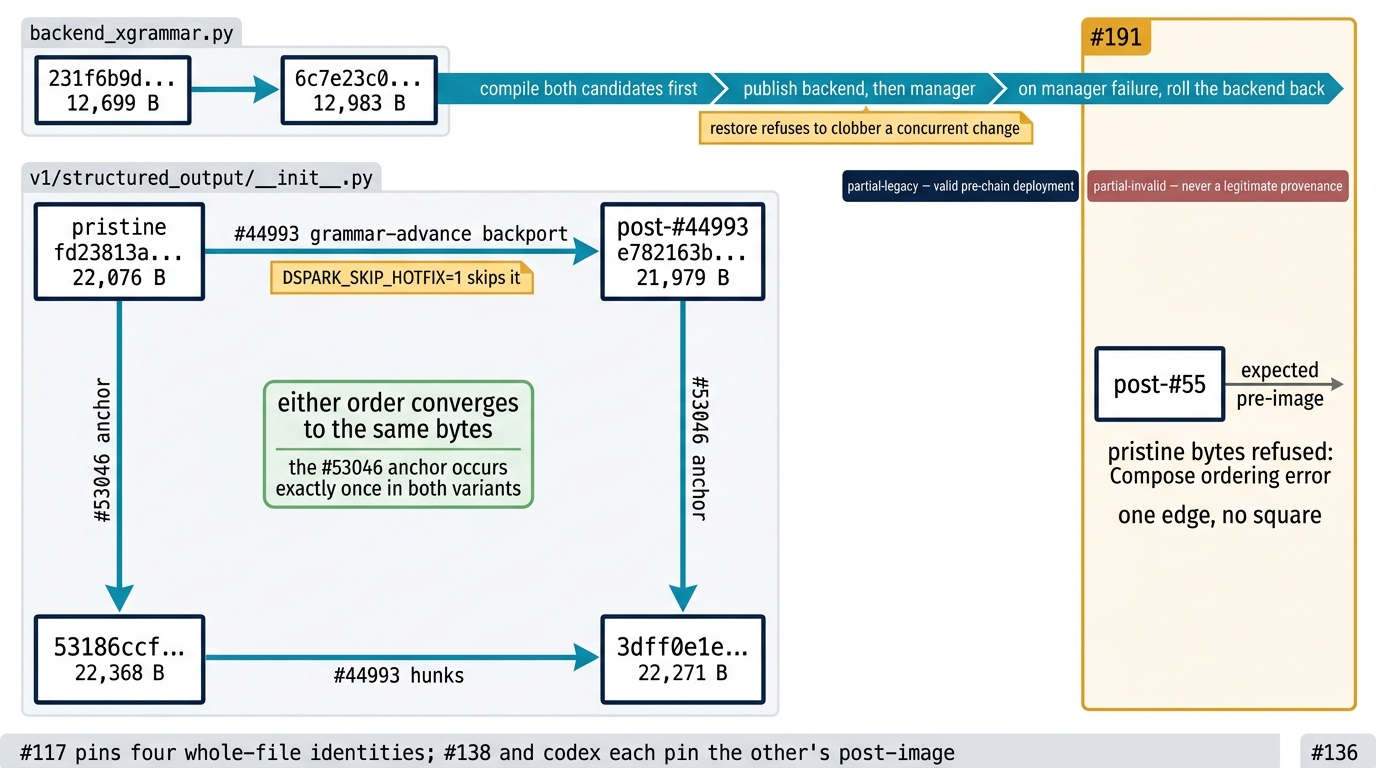
\includegraphics[width=\textwidth]{figures/ch06-multi-preimage.png}
\caption{Independent gating means every reachable boot order is a legitimate
pre-image. The \ghissue{136} chain's manager file can be met pristine
(\code{fd23813a}, 22{,}076\,B) or post-\ghissue{44993} (\code{e782163b},
21{,}979\,B) depending only on whether the operator booted with
\envvar{DSPARK_SKIP_HOTFIX}\code{=1}, so the patcher pins both with their
respective post-images, and CI proves constructively that applying the
\ghissue{44993} hunks and the \ghissue{53046} hunk in either order converges
to the same bytes. Because \ghissue{136} touches two files it also needs a
chain transaction: both candidates compiled before the first write, backend
published then manager, and a rollback that refuses to clobber a concurrent
change. Right: the contrast case --- issue \ghissue{191}'s pre-image is a
hard dependency, not a lattice.}
\label{fig:patch-multi-preimage}
\end{figure}

\section{Lifecycle: sync, recreate, upgrade}
\label{sec:patches-lifecycle}

Multiple pre-images cover what a patcher may meet on one machine --- but the
deployment runs two, and both ranks must run identical trains. The launcher
\code{scp}s every patcher
to the worker's canonical \repofile{patches/} path before starting anything.
The CI wiring gates check the worker sync list per patch, including one
sharp edge: the \repofile{vision_exp/} directory sync must
\code{rm -rf} the remote directory before \code{scp -r} so stale trees
cannot nest inside themselves.

Flag flips follow the recreate-versus-restart doctrine of
\Cref{sec:patches-strategy}: a real two-node stop/remove/start, never
\code{restart}.

The image-upgrade policy closes the loop. Because enabled mode pins exact
bytes, ``enabled mode intentionally rejects even a newer upstream file'' ---
a deliberate choice. On an image upgrade the operator leaves the flag off
until the pins are re-derived, rather than letting a patcher fuzzily apply to
code it has never seen. And when upstream merges the fix, the patch is
removed \emph{whole}: for \ghissue{136}, ``once the image incorporates
PR \ghissue{52805}, remove this patcher, flag, fixtures/tests,
sync/preflight, and documentation together.''

The repository has exercised this exit path end to end. When upstream reverted the
\ghissue{50004} adaptive-top-k backport (\ghissue{51318}, for the
capture-stride corruption told in \Cref{ch:bugs}), the fork removed its port
whole, giving back the claimed 1.0\,\% end-to-end gain. Because the
pinned image's stock code is exactly the pre-\ghissue{50004} state, removal
restored the upstream post-revert state precisely. Upstream later re-landed
the optimization capture-safely (\ghissue{52823}, 2026-08-21), but with no
capture-safe variant portable to this image, the fork stayed on stock. The
CI transaction inventory --- the frozen record of every production hunk ---
records the removal explicitly, so test coverage could not silently shrink
around the deleted patch.

\section{CI enforcement: the wiring gate and its honest limits}
\label{sec:patches-ci}

None of the above discipline survives contact with contributors unless it is
enforced mechanically. The gate that follows has two halves worth keeping
apart: what it proves about the recipe --- wiring, byte transformations,
transaction semantics, ordering --- and what it structurally cannot prove,
because it never executes a GPU kernel or runs on the arm64 platform the
patches ultimately land on. \repofile{scripts/ci-validate.sh} (562 lines, the same
script GitHub Actions runs) is that enforcement: shell syntax over every
script, \code{py_compile} over every patcher \emph{and} every test, roughly
33 hermetic CPU suites, and then a battery of regression-guard greps that
read like the project's institutional memory --- nearly every failure message
names the incident that created it.

The structural core is the four-part patch-governance invariant, demanded per
patch: \emph{default-off env gate, exact-\code{1} comparison,
\code{|| exit 1} fail-closed invocation, worker \code{scp} sync}. Each of
the four properties is independently grepped for every gated hotfix, plus
per-patch specifics (the \ghissue{138} worker env line must appear
exactly four times; the redaction patch must sit outside the skippable loop).
Greps are backed by behavior: the wiring suites extract the \emph{real}
compose entrypoint lines and execute them against recording \code{python3}
stubs, proving that enabled steps run in order, that any step's failure
blocks all later steps and the service \code{exec}, and that a flag value of
anything but exact \code{1} never invokes a gated patcher.

The strongest provenance claim in the repository anchors the hermetic patch
suites: the \ghissue{117} post-image fixture is verified equal, by Git
blob SHA-1, to the official upstream merge. Around that anchor, the suites
rest on fixture triangulation. Checked-in fixtures of the pinned vLLM
sources are locked by SHA-256 and byte length, and three independent legs
--- fixture hashes, the patcher's own pinned constants, and hunk literals
duplicated inside the test --- must agree. Replacing the test-local hunks in
the stock fixture must reproduce the post fixture byte-for-byte, so fixture,
patcher, and test check one another
(\Cref{fig:patch-fixture-triangulation}).

The transaction harness goes further. It parses the production \code{patch(...)}
calls out of each shell script's heredoc via AST, generates synthetic trees
from them, and pins every hunk in a frozen inventory (so deleting a production
hunk cannot shrink its own coverage). It then injects faults --- a
monkey-patched \code{os.replace} that fails at the $N$-th call, corrupted
re-reads, a \code{KeyboardInterrupt} mid-verification --- to prove rollback
restores bytes \emph{and} permission bits in reverse order.

The limits are stated as plainly as the guarantees. The gate is CPU-only:
``Does NOT run the live 2$\times$ Spark serve, decode bench, or
tool-eval-bench.'' It executes no GPU kernel and never touches the arm64
GB10 platform the patches ultimately run on, so it can prove the \emph{recipe}
--- wiring, byte transformations, transactions, fail-closed semantics ---
but not the runtime behavior of the patched kernels. The repository is careful not
to blur that line: the \ghissue{136} changelog entry explicitly ``does not
claim the live incident closed'' until a two-rank canary and log/health gate
pass, and the \ghissue{141} entry lists exactly which live validations remain
outstanding. Live evidence belongs to the verification scripts and canaries
of \Cref{ch:measurement}; CI's job is to make sure that what boots is exactly
what was reviewed.

\begin{figure}[htbp]
\centering
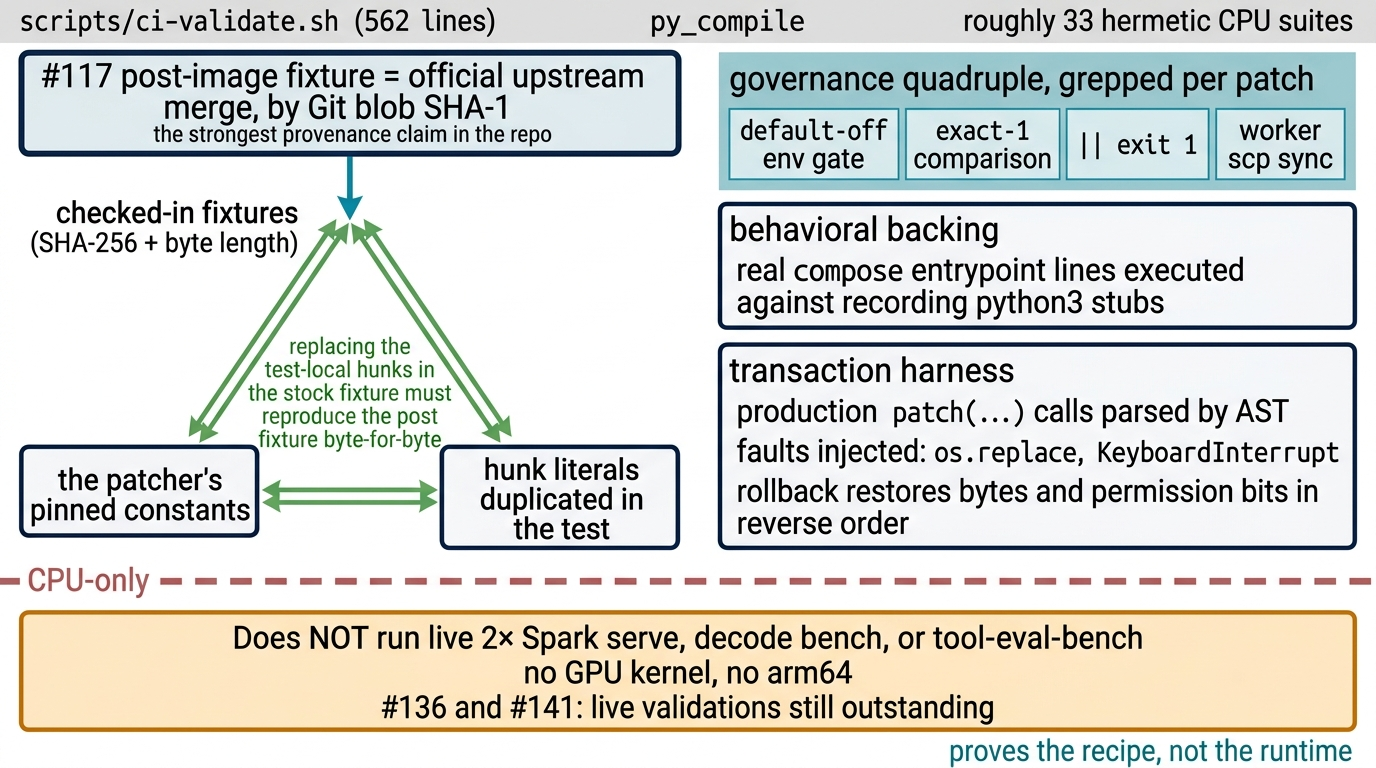
\includegraphics[width=\textwidth]{figures/ch06-fixture-triangulation.png}
\caption{The hermetic patch suites close on themselves: fixture hashes, the
patcher's pinned constants, and hunk literals duplicated inside the test must
all agree, and replacing the test-local hunks in the stock fixture must
reproduce the post fixture byte-for-byte --- anchored externally by the
\ghissue{117} post-image fixture verified equal by Git blob SHA-1 to the
official upstream merge. Around that core, the governance quadruple is
grepped per patch and backed behaviorally by executing the real compose
entrypoint lines against recording stubs, while the transaction harness
injects faults to prove reverse-order rollback of bytes and permission bits.
Below the dashed line is what a CPU-only gate structurally cannot reach: no
GPU kernel, no arm64 GB10, and no claim that a live incident is closed.}
\label{fig:patch-fixture-triangulation}
\end{figure}

A digest looked, at the start of this chapter, like the end of a provenance
question. It is the beginning of one. What a rank actually runs is that
digest plus a corpus of forty-odd transformations, applied in whatever order
the operator's flags select, into a writable layer that outlives every
\code{docker restart} --- which is why the hard engineering here lives in the
invocation and the pre-image sets rather than in the diffs. The unit of trust
shifted accordingly: not ``is this patch correct?'' but ``is every reachable
provenance enumerated, and is every failure of this patch reachable?'' A fix
nobody can prove was applied, and a failure nothing can surface, are the same
thing as no fix at all.

\FloatBarrier
\section*{Takeaways}
\begin{itemize}
\item Pinning an upstream image by manifest digest and patching it at
  container start buys byte-exact provenance, small reviewable diffs, and
  rollback-by-recreate --- at the price of writable-layer hidden state.
  Restart is not rollback; every flag change is a two-node recreate.
\item Match verification rigor to blast radius --- anchor+marker replaces for
  additive tweaks, whole-script transactions for multi-hunk backports, and
  SHA-256 pre/post-image (or AST-extracted-method) locks with version pins
  wherever drift could mean silent wrong behavior --- and give every family
  the same mechanics: never write before everything validates and compiles in
  memory, publish atomically, re-verify what you published, roll back in
  reverse order, and make a failed rollback loud, not quiet.
\item Gate opt-ins on the exact string \code{"1"}, default anything unproven
  to off, and chain every step with \code{|| exit 1}. Bare semicolons in an
  entrypoint are a latent incident (issue \ghissue{107}): a masked patch
  failure means serving stale code silently. And make \code{--status} tell
  the truth behaviorally, not by marker grep --- ``a hotfix whose
  \code{--status} lies is worse than no hotfix.''
\item Independent opt-ins that touch the same file must pin every legitimate
  pre-image (pristine \emph{and} post-sibling-patch) and prove order
  convergence; multi-file patches need chain transactions whose rollback
  refuses to clobber concurrent changes. Plan the exit on the way in, too:
  enabled mode rejects even a newer upstream file, and when upstream merges
  the fix, the patcher, flag, fixtures, tests, sync, and docs are removed
  together.
\item Enforce the governance quadruple --- default-off, exact-\code{1},
  fail-closed, worker-synced --- mechanically in CI, and be explicit about
  what a CPU-only gate cannot prove: no GPU, no arm64, no live incident
  closure.
\end{itemize}

\chaptertransition{A patch train is a machine for applying answers, and it
says nothing about the questions. Every one of those forty-odd corrections
was bought by an incident, and so was the machinery itself --- the byte pins,
the behavioral status checks, the refusal to guess at a pre-image are each
the scar of a specific failure that a looser method had already let through.
So the next chapter opens the museum: what actually went wrong, filed as
symptom, root cause, fix, and evidence. It begins with the incident that
gives the whole catalog its signature --- eight streams at 32K in which the
worst decode lane fell to 0.36 tokens per second while the preemption
counter, and every other counter an operator thinks to watch, read exactly
zero.}
